\documentclass{article}
\usepackage[T1]{fontenc}
\usepackage[utf8]{inputenc}
\usepackage{amsmath,amssymb}
\usepackage{tikz}
\usepackage{tikzsymbols}
\usepackage{tabularx}
\usepackage{lmodern}
\usepackage{xcolor}
\usepackage{algorithm2e}
\usepackage{titlesec}
\titlelabel{\thetitle.\ Aufgabe}
\usetikzlibrary{arrows,automata}
\setlength\parindent{0pt}

\begin{document}

\begin{center}
  \Large{Informatik D -- Klausur 2013 -- Batman \& Robin}

  \large{Sebastian Höffner, Andrea Suckro, Judith Kemper}
\end{center}

\section{}
\begin{itemize}
	\item reguläre Sprache: deterministisch endlicher Automat
  \item kontextfrei: Kellerautomat
  \item det. kontextfrei: deterministischer Kellerautomat
  \item kontextsensitiv: linear beschränkter Automat
\end{itemize}

\section{}
An den Kanten für eine Turingmaschine steht $A/B,C$. $A$ ist das Zeichen, was wir von dem Band lesen ($\in \Gamma$), B ist was wir auf das Band schreiben (ebenfalls $\in \Gamma$). $C$ ist die nächste Aktion, die die Turingmaschine ausführen soll, wobei $C \in \{R,L,S\}$ (Links,Rechts,Stopp). 

\section{}
mindestens notwendige Sprachklasse:
\begin{enumerate}
	\item regulär
  \item rekursiv aufzählbar
  \item deterministisch kontextfrei
  \item regulär
\end{enumerate}

\section{}
Regulärer Ausdruck: $(c|d)(c|d)cb^*a$

\section{}
\begin{align*}
S&\rightarrow 02A20 | 020\\
A&\rightarrow 0A0 | 1A1 | 2A2 | B\\
B&\rightarrow 0|1|2
\end{align*}

\section{}
Kellerautomat für die reguläre Sprache $\{a^{3i}b|i\geq0\}$:

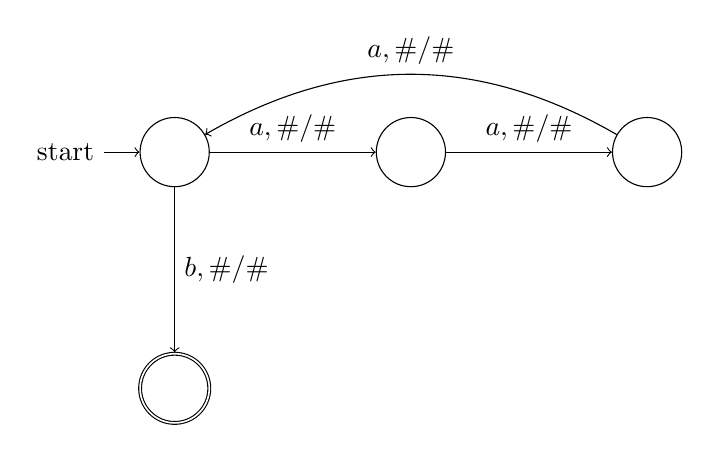
\begin{tikzpicture}[->, auto, node distance=3cm]
	\node[initial,state]   (A) {};
  \node[state,accepting] (B) [below of = A] {};
  \node[state]           (C) [right of = A] {};
  \node[state]           (D) [right of = C] {};
  \path (A) edge [] node {$b,\#/\#$} (B)
            edge [] node {$a,\#/\#$} (C)
        (C) edge [] node {$a,\#/\#$} (D)
        (D) edge [bend right, above] node {$a,\#/\#$} (A);
\end{tikzpicture}

\section{}
Schritt 1 (A-Variablen für jeden Zustand erstellen):
\begin{align*}
A_1&\rightarrow aA_4\\
A_2&\rightarrow cA_4|cA_1\\
A_3&\rightarrow \epsilon\\
A_4&\rightarrow bA_4 | aA_2 | dA_3 |d
\end{align*}
Schritt 2 (reguläre Grammatik daraus bauen):
\begin{align*}
S&\rightarrow aA\\
A&\rightarrow bA |aB|d\\
B&\rightarrow cA |cS
\end{align*}

\section{}
Pumping Lemma für reguläre Grammatik heißt: Für eine Mindestwortlänge $n$ gibt es für jedes Wort einer Sprache $L$ eine Zerlegung in $uvw$ mit $|v|\geq 1$,$|uv|\leq n$,$uv^*w \in L$. Zeigen wir nun für ein Wort aus L $z=a^nb^{n+n}a^n$,$|z|>n$, dass es keine Zerlegung gibt. Da $|uv|\leq n$ gelten muss wissen wir, dass $uv$ nur a's enthält. Sei $l=|v|\geq 1$. Dann ergibt sich für unsere Zerlegung $a^{n-l}a^lb^{2n}a^n$. Da $uv^*w \in L$ gelten muss, prüfen wir das Wort $uw = a^{n-l}b^{2n}a^n$. Nun sind allerdings nicht $i+j$ b's vorhanden, da $2n\neq n-l+n = 2n-l$. Somit ist dieses Wort $\notin L$- die Sprache ist also nicht regulär!

\section{}
Der Fehler liegt direkt in der ersten Zeile bei "Für alle Teilmengen $T'$...". Im Post'schen Korrespondenzproblem kann man jedoch Teile beliebig oft benutzen und damit kann man nicht einfach alle Teilmengen aufzählen, sondern es gibt unendlich viele.



\end{document}